%!TEX encoding = UTF-8 Unicode
\documentclass[12pt]{article} 
\usepackage[left=0.75in,top=0.7in,right=0.75in,bottom=0.3in]{geometry} % Document margins
\usepackage{CJK}
\usepackage{graphicx}
\usepackage{sidecap}
\usepackage{mathtools}
\usepackage{mathrsfs}
\usepackage{amssymb}
\usepackage{hyperref}

\makeatletter
\renewenvironment{itemize}
{\list{$\bullet$}{\leftmargin\z@ \labelwidth\z@ \itemindent-\leftmargin
\let\makelabel\descriptionlabel}}
{\endlist}
\makeatother

\begin{CJK}{UTF8}{bsmi}
\title{\textbf{Homework3 / Back propagation for functions approximation}}
\author{\textbf{李豪韋 (HW-Lee) ID 103061527}}
\date{}

\begin{document}
\vspace*{-60pt}
    {\let\newpage\relax\maketitle}

\section*{Overview}
\vspace{-20pt}
\noindent\makebox[\linewidth]{\rule{\textwidth}{0.4pt}}
\vspace{5pt}

In concepts of linear filtering for line fitting, we know that linear filtering can general learn a model linearly mapping input sets to desired output sets, but cannot deal with non-linear relation very well without lifting functions. (e.g. we cannot make the model infinitely approach the quadratic function without adding $x^2$ as a feature.) Therefore, an idea of cascading multiple stages of neural layers which contains several neurons as a learning system is suggested. Theoretically, it will work because the model complexity is increased as we apply more neurons or more layers, and this project is aimed at verifying its feasibility and discussing some issues of implementation during this work.

For purposes of easily usability and highly flexibility for programming/simulation, I constructed a simple framework consisting of some objects needed in a neural network. (e.g. Neurons, Neural Layers, Neural Nets, and Learning System) Because of limited pages of the report, only the relatively important(or the most important) part will be described in the report, and the more detailed information of the framework is publicly available on \href{https://github.com/HW-Lee/2015-NN-Homeworks/tree/master/HW03}{$\mathsf{https://github.com/HW}$-$\mathsf{Lee/2015}$-$\mathsf{NN}$-$\mathsf{Homeworks/tree/master/HW03}$}.

\section*{Implementation}
\vspace{-20pt}
\noindent\makebox[\linewidth]{\rule{\textwidth}{0.4pt}}

\begin{enumerate}
	\item {\bf Objects and Functions}
	\begin{itemize}
		\item {\bf Node} is a point with a certain value, used for calling value with reference.
		\item {\bf Neuron} is an unit in a neural net with some arithmetic functions and several I/O {\bf Nodes}.
		\item {\bf NeuralLayer/NeuralNet} is a container consisting of a couple of {\bf Neurons}/{\bf NeuralLayers}.
		\item {\bf TrainingSystem} is a learning system controlling how to change the weights of a net when training instances are given.
	\end{itemize}
	
	\vspace*{-2.5em}
	\begin{figure}[ht]
		\centering
		\hspace*{-6em}
		\begin{minipage}[b]{.45\linewidth}
			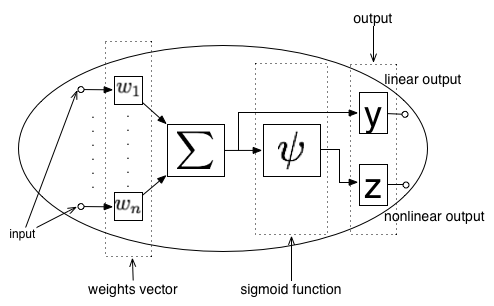
\includegraphics[width=10cm, height=4.5cm]{../res/Neuron.png}
			\caption{Structure of a Neuron}
		\end{minipage}
		\hspace{3em}
		\begin{minipage}[b]{.54\linewidth}
			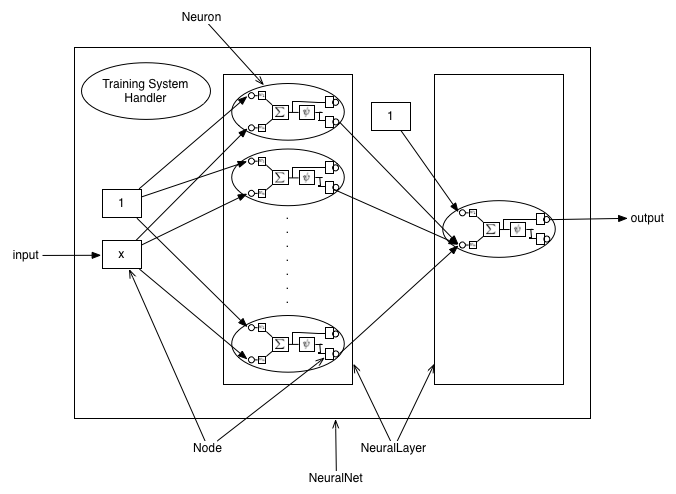
\includegraphics[width=12cm, height=6.5cm]{../res/NeuralNet.png}
			\caption{Structure of a NeuralNet with a hidden layer}
		\end{minipage}
	\end{figure}
	
	\newpage
	
	\begin{SCfigure}
		\centering
		\vspace*{-2em}
		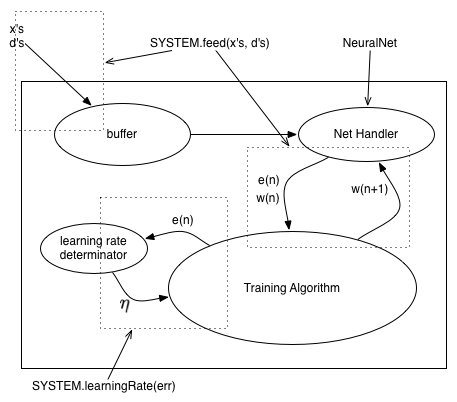
\includegraphics[scale=.57]{../res/TrainingSystem.png}
		\caption{The operation flow between a {\bf Neural Net} and a {\bf Training System}: 1) a number of instances will be stored in the buffer and sent one-by-one, 2) the difference between output value and desired value will be generated, 3) the {\bf Neural Net} and the difference will be sent to algorithm processor, 4) algorithm will get an appropriate learning rate from learning rate determining function with the error, 5) update the new weights of the {\bf Neural Net}, and then 6) repeat the process until the buffer is empty.}
	\end{SCfigure}
	
	\vspace*{-1.5em}
	\item {\bf Process}
	\begin{itemize}
		\item {\bf Feed an instance and compute the error}
		\item {\bf Compute all local gradients $\delta$'s}
		\item {\bf Update all weights based on outputs of each stage and local gradients}
	\end{itemize}
\end{enumerate}

\begin{figure}[ht]
	\vspace*{-1em}
	\centering
	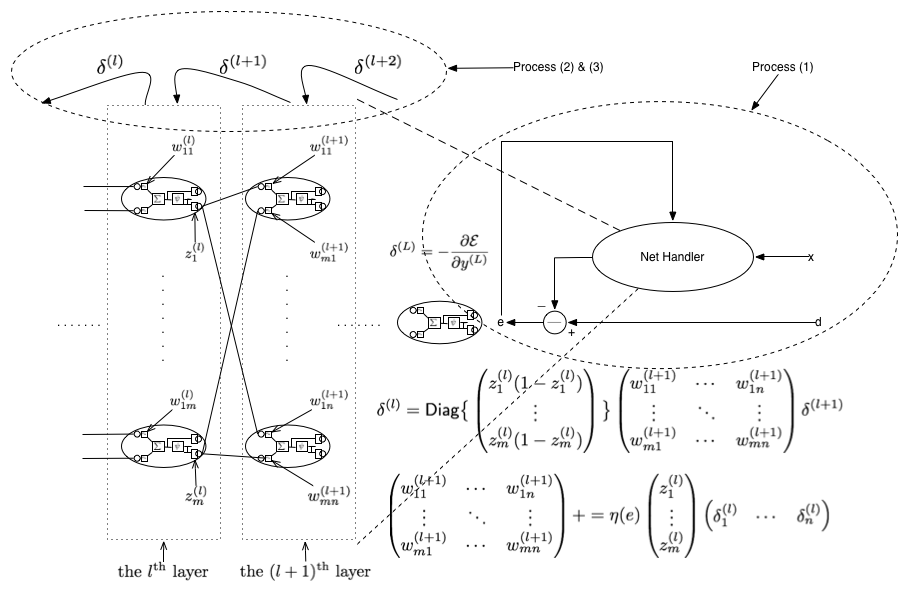
\includegraphics[scale=.52]{../res/BPAlgoDiagram.png}
	\caption{Process of back propagation algorithm: a more detailed demo of "Training Algorithm" block in the Figure 3}
\end{figure}

\newpage
\section*{Results}
\vspace{-20pt}
\noindent\makebox[\linewidth]{\rule{\textwidth}{0.4pt}}

\vspace{2em}
\begin{figure}[ht]
	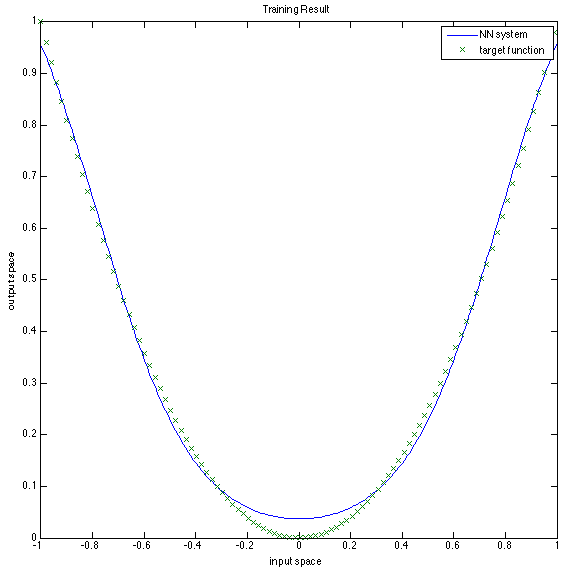
\includegraphics[scale=.45]{../res/result_quadratic_nN2.png}
	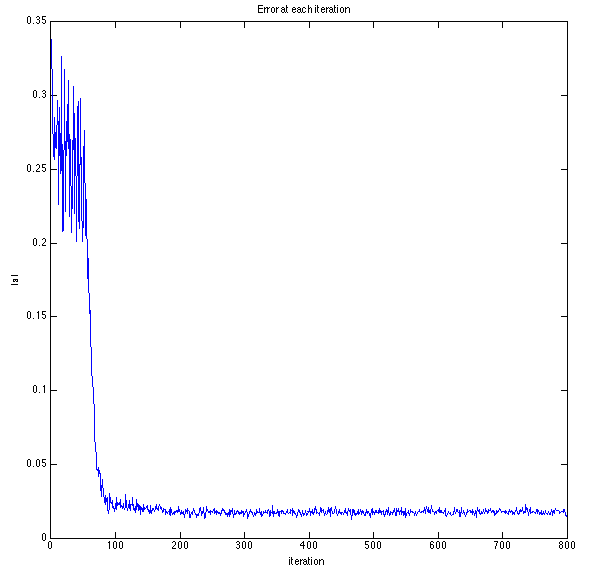
\includegraphics[scale=.45]{../res/absErr_quadratic_nN2.png}
\end{figure}

\begin{figure}[ht]
	\vspace*{-2.2em}
	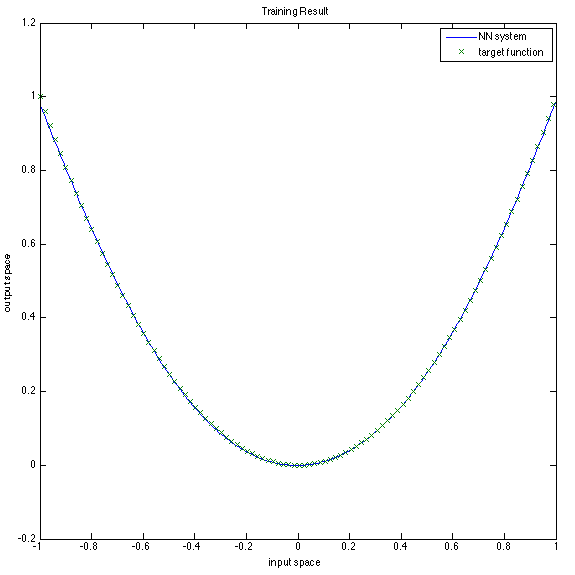
\includegraphics[scale=.45]{../res/result_quadratic_nN5.png}
	\hspace*{.5em}
	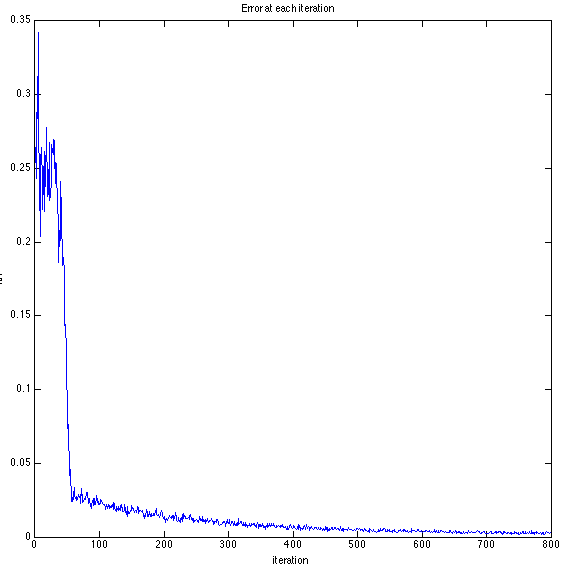
\includegraphics[scale=.45]{../res/absErr_quadratic_nN5.png}
	\caption{Training results and absolute error at each iteration (50 instances/iteration) with two different number of hidden neurons: 1) 2 hidden neurons upper, and 2) 5 hidden neurons lower}
\end{figure}

\newpage
\section*{Discussion}
\vspace{-20pt}
\noindent\makebox[\linewidth]{\rule{\textwidth}{0.4pt}}

\begin{enumerate}
	\item Does initialization matter?
		\begin{flushleft}
			In practice, yes. Note that this algorithm CANNOT use zero initialization because the local gradients will be always zero. (see Figure 4)
		\end{flushleft}
	\item Does randomization matter?
		\begin{flushleft}
			The randomly selected samples are relatively irrelevant to the result after a sufficiently large iterations. Instead of it, the range of samples 
			is a key reason determining training efficiency.
		\end{flushleft}
	\item How does the learning rate affect the system's behavior?
		\begin{flushleft}
			It affects whether the system will finally get converged, how fast it gets converged, and how many iterations it requires to get converged.
		\end{flushleft}
	\item Does the system always converge to the same set of weights or does the system sometimes 'get stuck' in a sub-optimal region 
		in the weight space? \\ \makebox{} \\
		%\begin{center}
			\hspace*{-6em}
			\begin{tabular}{|c|c|c|c|c|c|}
				\hline
				 & $n^{(1)}_1$ & $n^{(1)}_2$ & $n^{(1)}_3$ & $n^{(1)}_4$ & $n^{(1)}_5$ \\
				\hline
				$b$ & $-1.55 \pm 0.90$ & $-1.65 \pm 0.90$ & $-0.81 \pm 1.81$ & $-0.06 \pm 2.67$ & $-1.20 \pm 0.78$ \\
				\hline
				$x$ & $1.16 \pm 1.08$ & $1.43 \pm 1.11$ & $-0.07 \pm 1.92$ & $0.04 \pm 2.56$ & $-0.76 \pm 0.86$ \\
				\hline
				 & $w^{(2)}_{11}$ & $w^{(2)}_{21}$ & $w^{(2)}_{31}$ & $w^{(2)}_{41}$ & $w^{(2)}_{51}$ \\
				\hline
				 & $0.63 \pm 1.85$ & $1.42 \pm 1.22$ & $1.21 \pm 1.58$ & $1.64 \pm 1.45$ & $0.48 \pm 1.47$ \\
				\hline
			\end{tabular}
			\hspace*{0em}
			\begin{tabular}{|c|c|c|}
				\hline
				 & $n^{(1)}_1$ & $n^{(1)}_2$ \\
				\hline
				$b$ & $-4.19 \pm 0.01$ & $-4.19 \pm 0.01$ \\
				\hline
				$x$ & $5.38 \pm 0.02$ & $-5.39 \pm 0.02$ \\
				\hline
				 & $w^{(2)}_{11}$ & $w^{(2)}_{21}$ \\
				\hline
				 & $1.24 \pm 0.02$ & $1.24 \pm 0.01$  \\
				 \hline
			\end{tabular} \\ \\
		%\end{center}
		The above table shows 10 sets of final weights after $800 \times 50$ instances learning the quadratic function with 5/2 hidden neurons. 
		According  to the table, the answer is NOT REALLY.
	\item How well does your system learn a different function, say $y=\cos^2(\frac{\pi}{2}x)$, $y=\sin(kx)$, $y=|x|$, and $y=\sqrt{|x|}$?
	\begin{figure}[ht]
		\hspace*{-2.9em}
		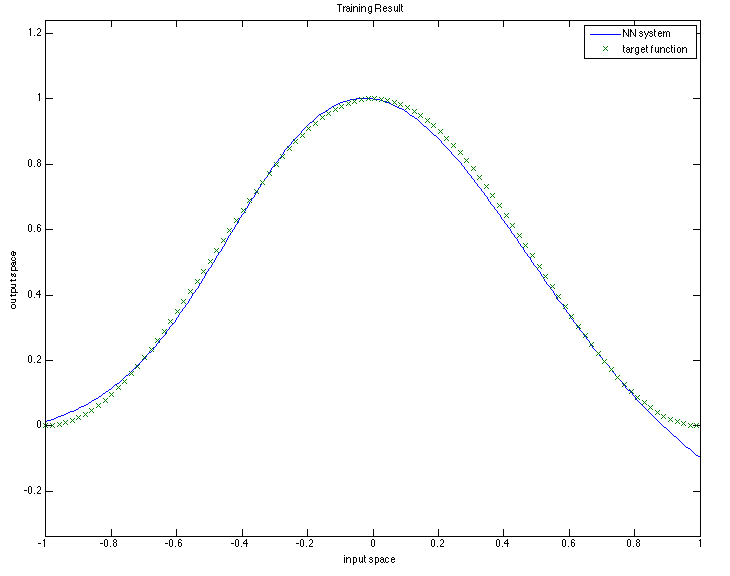
\includegraphics[scale=.19]{../res/result_cos2_nN5.png}
		\hspace*{-1em}
		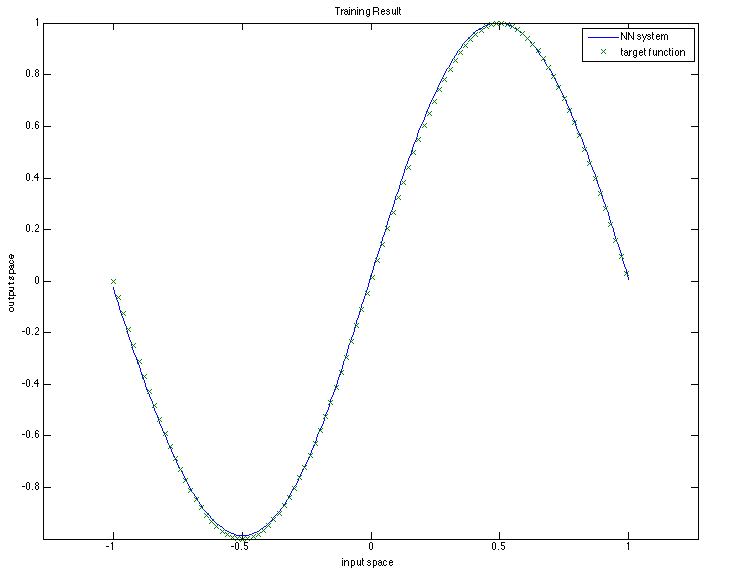
\includegraphics[scale=.19]{../res/result_sin_nN5.png}
		\hspace*{-1em}
		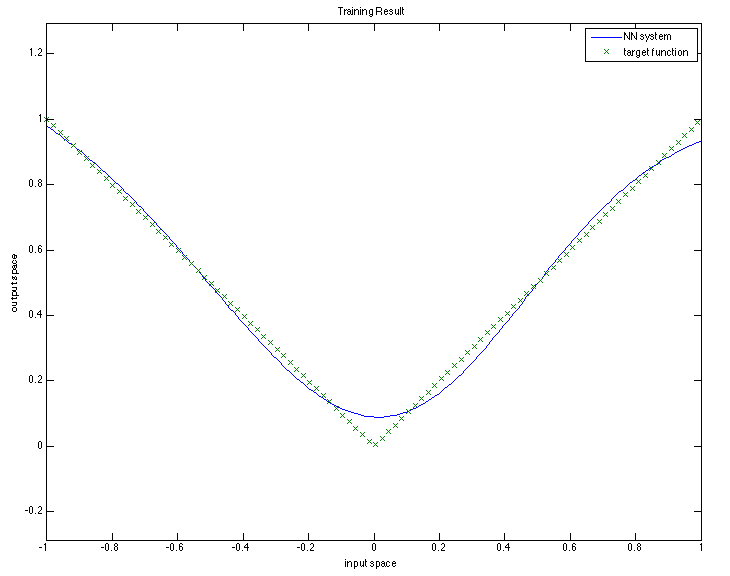
\includegraphics[scale=.19]{../res/result_abs_nN5.png}
		\hspace*{-1em}
		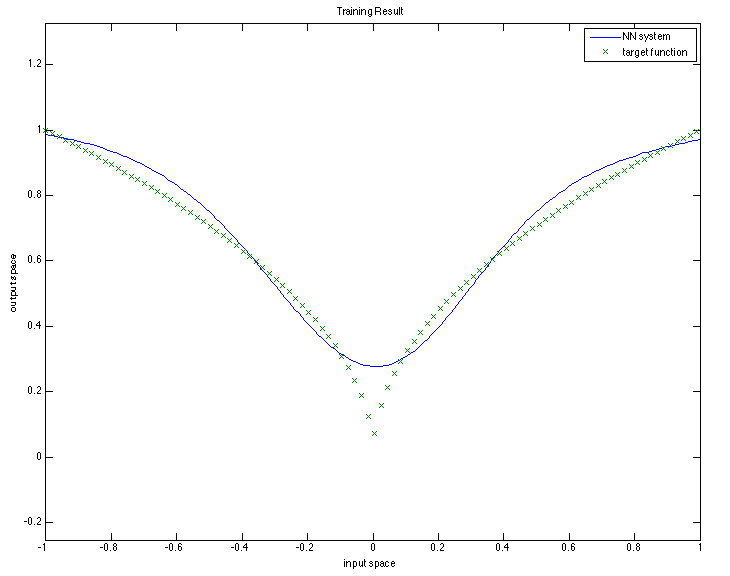
\includegraphics[scale=.19]{../res/result_abs_sqrt_nN5.png}
		\caption{NN system training results of different target functions: 
		$y=\cos^2(\frac{\pi}{2}x)$, $y=\sin(\pi x)$, $y=|x|$, $y=\sqrt{|x|}$ (from left to right) }
	\end{figure}
	\item Continuing from Q3, does it help to increase the number of hidden neurons if the system suggested from the assignment sheet 
		does not learn a function well?
		\begin{flushleft}
			In general, yes. (see Additional Discussion section)
		\end{flushleft}
\end{enumerate}

\newpage
\section*{Additional Discussion: Why does it (multi-layer) work?}
\vspace{-20pt}
\noindent\makebox[\linewidth]{\rule{\textwidth}{0.4pt}}

\begin{enumerate}
	\item Describe the sigmoid function, says generally {\bf logistic function}, in another way.
	\vspace*{-.5em}
	\begin{align*}
		\phi(x) &= \frac{1}{1+e^{-x}} = \lim_{n \to \infty} \displaystyle\sum_{i=0}^{n} \frac{\phi^{(i)}(x_0)}{i!} (x-x_0)^{i} = 
		\frac{1}{2} + \lim_{n \to \infty} \displaystyle\sum_{i=1}^{n} a_i (x-x_0)^{i}  \\ 
		&\text{, where } a_i = \frac{\phi^{(i)}(x_0)}{i!}
		, \,\,  \phi^{(n)}(x) = \phi^{(n-1)}(x)(1-2\phi(x)) - \sum_{i=1}^{n-2} C^{n-1}_i \phi^{(n-1-i)}(x)\phi^{(i)}(x) \,\, \forall \, n > 2 \\	
		%\phi^{(n+1)}(x) &= \phi^{(n)}(x)(1-2\phi(x))-2\phi^{(n-1)}(x)\phi^{(1)}(x) - 
		%\sum_{i=1}^{n-2} C^{n-1}_i \big( \phi^{(n-i)}(x)\phi^{(i)}(x)+\phi^{(n-1-i)}(x)\phi^{(i+1)}(x) \big) \\
		%2\phi^{(1)}(x)\phi&^{(n-1)}(x) + \sum_{i=1}^{n-2} C^{n-1}_i \big( \phi^{(n-i)}(x)\phi^{(i)}(x)+\phi^{(n-1-i)}(x)\phi^{(i+1)}(x) \big) \\
		%&= 2\phi^{(1)}(x)\phi^{(n-1)}(x) + \sum_{i=1}^{n-2} C^{n-1}_i \phi^{(n-i)}(x)\phi^{(i)}(x) +
		%\sum_{i=2}^{n-1} C^{n-1}_{i-1} \phi^{(n-i)}(x)\phi^{(i)}(x) \\
		%&=2\phi^{(1)}(x)\phi^{(n-1)}(x) + C^{n-1}_1 \phi^{(n-1)}(x)\phi^{(1)}(x) + C^{n-1}_{n-2}\phi^{(1)}(x)\phi^{(n-1)}(x) + 
		%\sum_{i=2}^{n-2} C^{n}_{i} \phi^{(n-i)}(x)\phi^{(i)}(x) \\
		%&= C^{n}_1 \phi^{(n-1)}(x)\phi^{(1)}(x) + C^{n}_{n-1}\phi^{(1)}(x)\phi^{(n-1)}(x) + 
		%\sum_{i=2}^{n-2} C^{n}_{i} \phi^{(n-i)}(x)\phi^{(i)}(x) = \sum_{i=1}^{n-1} C^n_i \phi^{(n-i)}(x)\phi^{(i)}(x) \\
		%\phi^{(n+1)}(x) &= \phi^{(n)}(x)(1-2\phi(x)) - \sum_{i=1}^{n-1} C^n_i \phi^{(n-i)}(x)\phi^{(i)}(x) \\
		\text{And we } &\text{can also obtain that: } \\
		\phi^{(n)}(x) &= \phi^{(n-1)}(x)(1-2\phi(x)) - \sum_{i=1}^{n-2} C^{n-1}_i \phi^{(n-1-i)}(x) \phi^{(i)}(x) < 2^{n-1} < n! 
		\text{ when $n$ is greater than 2} \\
		\implies &\text{If $n$ is sufficiently large, the expansion can even perfectly fit the closed form curve for any $x$ } \\
		&\text{and any $x_0$. Therefore, we can simply assume $x_0 = 0$ without loss of generality.}
	\end{align*}
	\item Under the structure constructed with a hidden layer with $m$ hidden neurons.
	\begin{align*}
		\text{For every} &\text{ hidden neuron: } \\
		z^{(1)}_i &= \phi(y^{(1)}_i) = \phi(w^{(1)}_{1i} + w^{(1)}_{2i}x) \approx 
		\frac{1}{2} + \displaystyle\sum_{k=1}^{N} a_k (w^{(1)}_{1i} + w^{(1)}_{2i}x)^{k} \text{, for some } N < \infty \text{, and $x_0 = 0$} \\
		&= b_{i0} + \sum_{k=1}^N b_{ik} x^{k} = \begin{pmatrix}b_{i0} & \cdots &b_{iN}\end{pmatrix} 
		\begin{pmatrix}1 \\ \vdots \\ x^N\end{pmatrix}
		\implies z^{(1)} = \begin{pmatrix}b_{10} & \cdots & b_{1N} \\ \vdots & \ddots & \vdots \\ b_{m0} & \cdots & b_{mN}\end{pmatrix}
		\begin{pmatrix}1 \\ \vdots \\ x^N\end{pmatrix} \\
		y^{(2)} &= z^{(1)T} \begin{pmatrix}w^{(2)}_{11} \\ \vdots \\ w^{(2)}_{m1}\end{pmatrix} \approx 
		\begin{pmatrix}1 & \cdots & x^N\end{pmatrix}
		\begin{pmatrix}c_0 \\ \vdots \\ c_N\end{pmatrix} = \sum_{k=0}^N c_k x^k \approx f(x)\\
		\implies &\begin{pmatrix}b_{10} & \cdots & b_{m0} \\ \vdots & \ddots & \vdots \\ b_{1N} & \cdots & b_{mN}\end{pmatrix}
		\begin{pmatrix}w^{(2)}_{11} \\ \vdots \\ w^{(2)}_{m1}\end{pmatrix} \approx
		\begin{pmatrix}c_0 \\ \vdots \\ c_N\end{pmatrix}
	\end{align*}
	\item Conclusions and Facts with reasons
	\begin{itemize}
		\item Multi-layer neural net does work because it works as an infinite order polynomial approximation with finite order polynomials.
		\item Theoretically, the more number of hidden neurons $m$, the better training performance we can get without considering computation 
			consumption and convergence issues. Because increasing $m$ is equivalently increasing $N$ and reducing the approximation error 
			of the expansion.
		\item The bias node is redundant in the second stage, so the bias node in the second stage has been removed in this project.
		\item The bias node is essential in the first stage because the net will only cover odd part ($x^{2n-1}$) and constant part if $b=0$. (i.e.
			$a_i \big|_{x_0=0} =0$, $\forall \, i$ is even.)
		\item In Result section, the error seems not to approach to zero because the chosen $N < \infty$. In addition, 5-hidden-neurons net also has
			lower static error, which proves that increasing $m$ can equivalently increase $N$ and than reduce the static error.
	\end{itemize}
\end{enumerate}

%\begin{align*}
%\delta^{(l)} = \mathsf{Diag}\big\{\begin{pmatrix}z^{(l)}_1(1-z^{(l)}_1) \\ \vdots \\ z^{(l)}_m(1-z^{(l)}_m)\end{pmatrix} \big\}
%\begin{pmatrix}w^{(l+1)}_{11} & \cdots & w^{(l+1)}_{1n} \\
%\vdots & \ddots & \vdots \\ w^{(l+1)}_{m1} & \cdots & w^{(l+1)}_{mn} \end{pmatrix} \delta^{(l+1)}
%\end{align*}

\end{CJK}
\end{document}